\section{Spread impact in price response functions}\label{sec:spread_impact}

To analyze the spread impact in price response functions, we use 47 foreign
exchange pairs from three different years (Appendix \ref{app:fx_pairs_spread}).
As we showed in Sect. \ref{sec:forex_overview}, due to the difference in the
position of the decimal points in the price between foreign exchange pairs, to
compare them we need to introduce a ``scaling factor'' with the purpose of
bringing the pip to the left of the decimal point. For example, the scaling
factor for the USD/JPY is $100$ and the one for the EUR/USD is $10000$.

The pip bid-ask spread is defined as \cite{micro_eff}
\begin{equation}
    s_{\textrm{pip}} = \left(a\left(t\right) - b\left(t\right)\right) \cdot
    \textrm{scaling factor}.
\end{equation}
With the $s_{\textrm{pip}}$ we can group the foreign exchange pairs and check
how the average strength of the price response functions on trade time scale
and physical time scale behave. For each pair we compute the pip bid-ask spread
in every trade along the market time. Then we average the spread during the
trade weeks in the different years. With this value we group the foreign
exchange pairs.

\begin{figure*}[htbp]
    \centering
    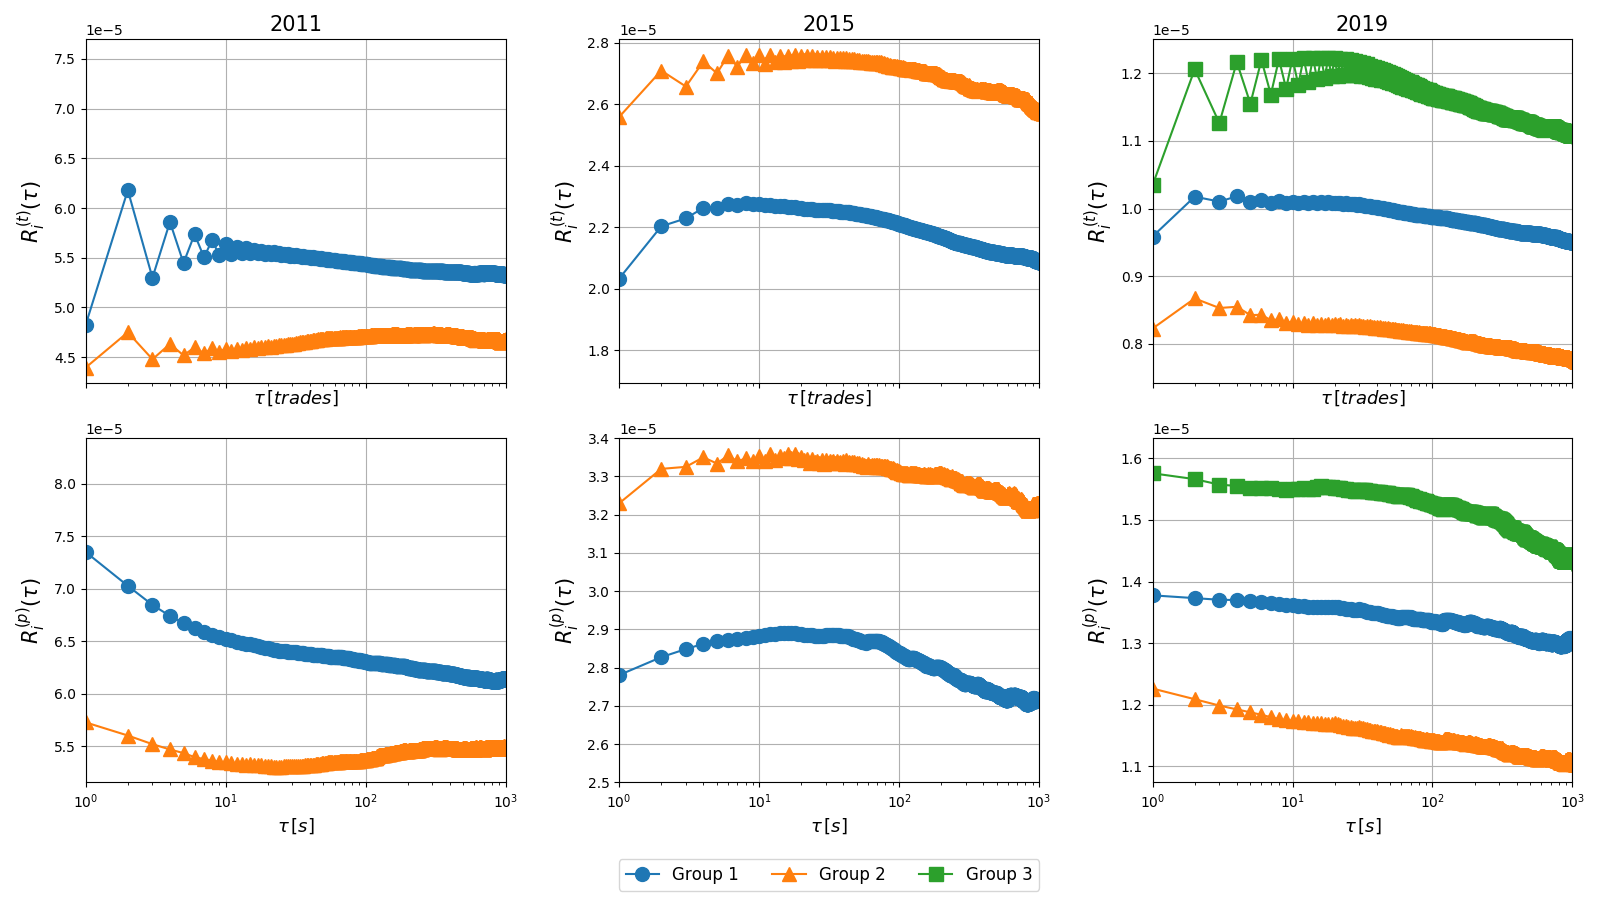
\includegraphics[width=\textwidth]{figures/05_spread_impact.png}
    \caption{Average price response functions
             $R^{\left(t\right)}_{ii}\left(\tau\right)$ versus time lag $\tau$
             on a logarithmic scale in trade time scale (Top) and
             $R^{\left(p\right)}_{ii}\left(\tau\right)$ excluding
             $\varepsilon^{\left(p\right)}_{i}\left(t\right) = 0$ versus time
             lag $\tau$ on a logarithmic scale in physical time scale (Bottom)
             for 47 foreign exchange pairs divided in representative groups in
             three different years (2011, 2015 and 2019).}
    \label{fig:spread_impact}
\end{figure*}

Depending on the year, we identify different number of groups according with
the pip spread $s_{\textrm{pip}}$. For the years 2011 and 2015, we use two
intervals to select the foreign exchange pairs groups ($s_{\textrm{pip}}<10$
and $10 \le s_{\textrm{pip}}$). In the year 2019 we use three intervals to
select the foreign exchange pairs groups ($s_{\textrm{pip}}<4$,
$4 \le s_{\textrm{pip}} < 10$ and $10 \le s_{\textrm{pip}}$). The detailed
information of the foreign exchange pairs, spread and the groups can be seen in
Appendix \ref{app:fx_pairs_spread}. With the groups of the stocks defined, we
average the price response functions of each group.

In Fig. \ref{fig:spread_impact} we show the average response functions for
the corresponding groups in three different years. From year to year the groups
can vary depending on the pip spread. The average price response function for
the pairs with smaller pip spreads (more liquid) have in average the weakest
signal in the figure for all the years and both time scales. On the other hand,
the average price responses for the pairs with larger pip spread (less liquid)
have in average the strongest signal for all the years in both time scales.

From Sect. \ref{sec:response_functions} we expect the increase-maximum-decrease
behavior. This behavior can be seen in the figures of the year 2015 for both
time scales and in the figure of the year 2019 in trade time scale. In these
figures the average price response functions follow an increase, reach a
maximum and then start to slowly decrease. For the other figures, on average,
the response functions start to decrease from the beginning.

The response in trade time scale seems to be noisier, with large changes in the
first time steps. This aggregate noise can be related with the crosses and
exotics pairs, who tend to fluctuate more.

For the years 2015 and 2019 in physical time scale, the
increase-maximum-decrease behavior is not that well defined as in Sect.
\ref{sec:response_functions} or as in the average response in trade time scale.
However, some groups tend to behave in the expected way. The groups that do not
follow the trend, seem to have a instantaneous high response that slowly
decrease with time. This behavior is mostly noticeable in the year 2019.

For the year 2011 in physical time scale, the increase-maximum-decrease shape
is not present. For both groups the response decrease almost immediately.

In the three plots, the foreign exchange market seems to have a global
influence over all the pairs in the corresponding years. A similar behavior
can be seen in correlated financial markets
\cite{my_paper_response_financial}.